\section{Задание 1 --- Анализ биоритмов в JavaScript}

Введите дату рождения

\begin{center} 
  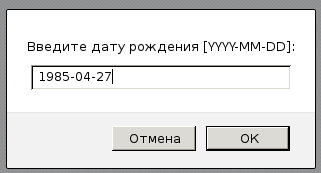
\includegraphics[width=9cm]{img/01.png}
\end{center}

Введите прогнозируемый год

\begin{center} 
  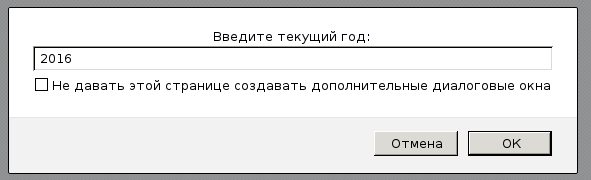
\includegraphics[width=9cm]{img/02.png}
\end{center}

Получившийся график:

\begin{center} 
  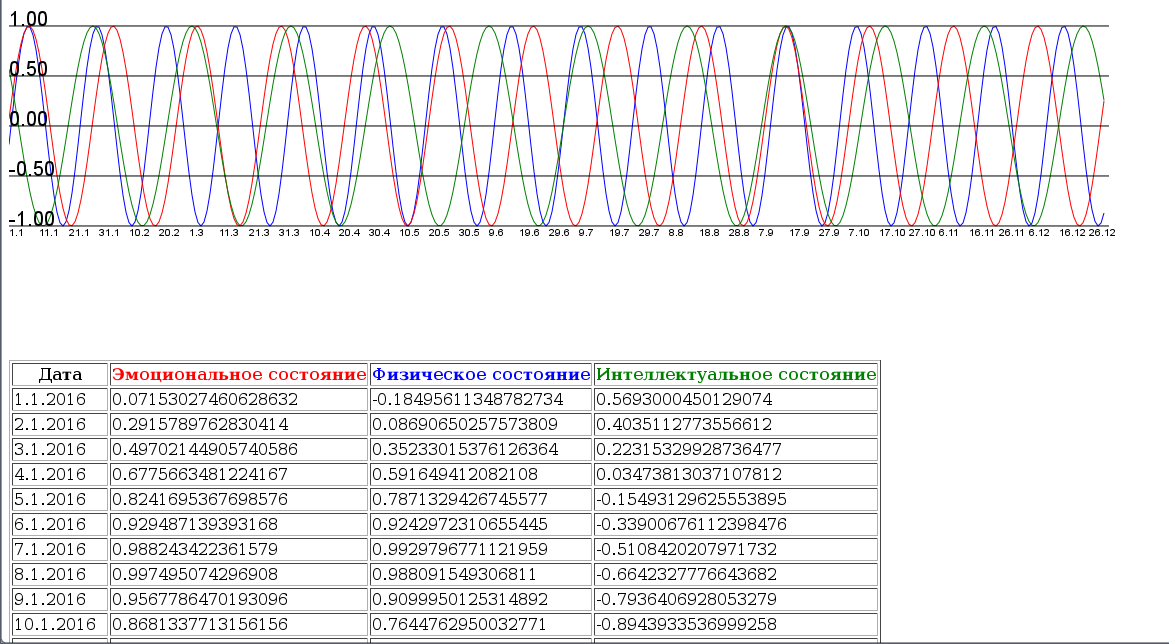
\includegraphics[width=15cm]{img/03.png}
  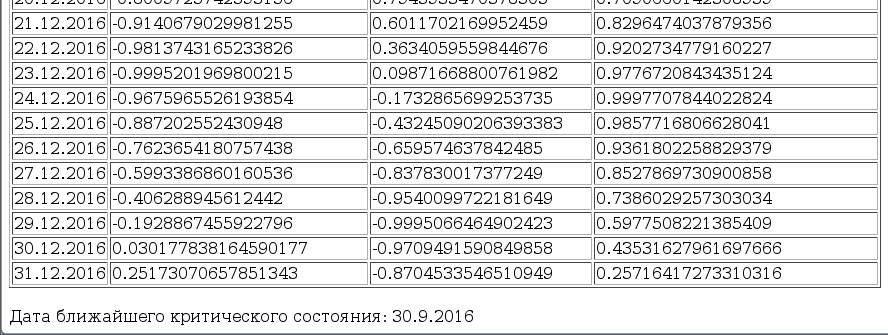
\includegraphics[width=15cm]{img/04.png}
\end{center}

Исходный код \verb|biorhythm.html|:

\begin{verbatim}
<!doctype html>
<html>
  <head>
    <title>Биоритмы</title>
    <meta charset='utf-8' />
  </head>
  <body>
    <canvas id='example'>Обновите браузер</canvas>
    <script>
      var str = prompt("Введите дату рождения [YYYY-MM-DD]:",
		       "1985-04-27");
      var birthDate = new Date(str);
      str = prompt("Введите текущий год: ", "2016");
      var currentYear = new Date(str);
      var changingDate = currentYear;
      var i = currentYear.getFullYear();
      var example=document.getElementById("example"),
	  ctx=example.getContext('2d');
      example.height=380; example.width=1200;
      var X=0, Y=0;
      Y = -Math.sin(2*3.14*(changingDate - birthDate)/
		    (24*60*60*1000*23))*100+150;
      ctx.strokeStyle="blue";
      ctx.moveTo(0,Y);
      ctx.font = "10px Arial";
      while ((changingDate.getFullYear()) == i) {
	  Y = -Math.sin(2*3.14*(changingDate - birthDate)/
			(24*60*60*1000*23))*100+150;
	  ctx.lineTo(X,Y);
	  if (X%30 == 0)
	      ctx.fillText(changingDate.getDate()+
			   "."+
			   (changingDate.getMonth()+
			    1),X,260);
	  changingDate.setDate(changingDate.getDate()+1);
	  X = X+3;
      }
      ctx.stroke();

      // Строим кривую эмоционального состояния
      ctx.beginPath();
      changingDate.setFullYear(i);
      changingDate.setMonth(0);
      changingDate.setDate(1);
      X=0;
      Y=0;
      Y = -Math.sin(2*3.14*(changingDate -
			    birthDate)/
		    (24*60*60*1000*28))*100+150;
      var criticalState = Y+
	  (-Math.sin(2*3.14*(changingDate - birthDate)/
		     (24*60*60*1000*23))*100+150) +
	  (-Math.sin(2*3.14*(changingDate - birthDate)/
		     (24*60*60*1000*33))*100+150);
      var criticalMonth = changingDate.getFullYear();
      var criticalDay = changingDate.getDate();
      ctx.moveTo(0,Y);
      ctx.strokeStyle="red";
      document.write("<table border=\"1\">");
      document.write(
	  "<tr><th>Дата</th><th>" +
	      "<font color=\"red\">Эмоциональное с"+
	      "остояние</font>" +
	      "</th><th><font color=\"blue\">Физи" +
	      "ческое состояние</font>" +
	      "</th><th><font color=\"green\">Инт" +
	      "еллектуальное состояние</font>"+
	      "</th></tr>");
      while ((changingDate.getFullYear()) == i) {
	  Y = -Math.sin(2*3.14*(changingDate - birthDate)/
			(24*60*60*1000*28))*100+150;
	  if (criticalState <
	      (Y+
	       (-Math.sin(2*3.14*(changingDate - birthDate)/
			  (24*60*60*1000*23))*100+150) +
	       (-Math.sin(2*3.14*(changingDate - birthDate)/
			  (24*60*60*1000*33))*100+150)))
	  {
	      criticalState = Y+
		  (-Math.sin(2*3.14*(changingDate - birthDate)/
			     (24*60*60*1000*23))*100+150) +
		  (-Math.sin(2*3.14*(changingDate - birthDate)/
			     (24*60*60*1000*33))*100+150);
	      criticalMonth = changingDate.getMonth();
	      criticalDay = changingDate.getDate();
	  }
	  ctx.lineTo(X,Y);
	  document.write("<tr><td>"+ changingDate.getDate() +
			 "." + (changingDate.getMonth() + 1)+
			 "." + changingDate.getFullYear() +
			 "</td><td>" + Math.sin(2*3.14*(changingDate -
							birthDate)/(24*60*60*1000*28)) +
			 "</td><td>" + Math.sin(2*3.14*(changingDate -
							birthDate)/(24*60*60*1000*23)) +
			 "</td><td>" + Math.sin(2*3.14*(changingDate -
							birthDate)/
						(24*60*60*1000*33)) +
			 "</td></tr>");
	  changingDate.setDate(changingDate.getDate()+1);
	  X = X+3;
      }
      document.write("</table>");
      document.write("<br>Дата критического состояния: " +
		     criticalDay + "." + (criticalMonth + 1) +
		     "." + i + "<br>");
      ctx.stroke();

      // Строим кривую интеллектуального состояния
      ctx.beginPath();
      changingDate.setFullYear(i);
      changingDate.setMonth(0);
      changingDate.setDate(1);
      X=0;
      Y=0;
      Y = -Math.sin(2*3.14*(changingDate - birthDate)/
		    (24*60*60*1000*33))*100+150;
      ctx.moveTo(0,Y);
      ctx.strokeStyle="green";
      while ((changingDate.getFullYear()) == i) {
	  Y = -Math.sin(2*3.14*(changingDate - birthDate)/
			(24*60*60*1000*33))*100+150;
	  ctx.lineTo(X,Y);
	  changingDate.setDate(changingDate.getDate()+1);
	  X = X+3;
      }
      ctx.stroke();

      // Рисуем оси координат
      ctx.beginPath();
      ctx.moveTo(0,150);
      ctx.strokeStyle="black";
      ctx.lineTo(1100,150);
      ctx.font = "20px Arial";
      ctx.fillText("0.00", 0, 150);
      ctx.moveTo(0,50);
      ctx.lineTo(1100,50);
      ctx.fillText("1.00",0,50);
      ctx.moveTo(0,100);
      ctx.lineTo(1100,100);
      ctx.fillText("0.50",0,100);
      ctx.moveTo(0,200);
      ctx.lineTo(1100,200);
      ctx.fillText("-0.50", 0,200);
      ctx.moveTo(0,250);
      ctx.lineTo(1100,250);
      ctx.fillText("-1.00", 0,250);
      ctx.stroke();
    </script>
  </body>
</html>
\end{verbatim}
